% questions.tex —— 2015 年·浙江卷·理科 · 题目内容片段（无答案）
% 由 tools/generate_projects.py 依来源总账自 2015/2015_数学真题_浙江理_试题.md 生成，勿手改（改源 MD 后重跑）


\gkpart{数学}

\begin{gktip}
\textbf{来源说明}：本题面依据固定源 PDF 全 2 页逐题核对（p1＝页 989：栏 1 标题与「一、选择题」1–5（第 5 题文字在栏 1 底部）；栏 2 第 5 题图与选项、6–8 与「二、填空题」9–11；栏 3 第 12–15 题与「三、解答题」16；p2＝页 990：栏 1 第 17 题（三棱柱）与第 18 题；栏 2 第 19 题（椭圆）；栏 3 第 20 题）。原卷为 \textbf{A3 横向三栏书刊合排}，阅读序＝左→中→右；\textbf{页脚仅印合订本书页页码 989／990}，\textbf{无页眉}；标题在栏 1 内排印。\textbf{全卷不印分值、不印题量}——三个节头逐字仅「一、选择题」「二、填空题」「三、解答题」；总分 150 为结构推断，\textbf{卷面无凭据}，本文件不作补写。

\textbf{源制作体系判定}（实测）：源\textbf{不是扫描件，而是 LaTeX（Computer Modern 系）重排产物}——\texttt{pdfimages -list} 零命中（全页无位图）；全卷 16 个嵌入字体：中文 \textbf{STSong／STHeiti}，拉丁与数学 \textbf{LMRoman12-Bold／LMRoman10-Regular／LMRoman10-Bold／LMRoman7-Bold、CMR10／CMR7／CMMI10／CMMI7／CMSY10／CMSY7／CMEX10／MSAM10}，另有 \textbf{CMMIB10（粗斜体）} 与 \textbf{TeX-vect10（向量箭头）}；\textbf{本卷无 STKaiti}（与同年的浙江文卷不同）。\textbf{CMMIB10 用于第 15 题的向量 \(\boldsymbol{e}_1,\boldsymbol{e}_2,\boldsymbol{b}\)（粗斜体）；TeX-vect10 仅出现在第 15 题范数式中的 \(\vec b\)}——源内同题向量记号混排（粗斜体为主、箭头一处），本库统一作粗斜体并在「存疑与登记」中说明。LJVORJ+CMMI7、NBEQIK+CMMIB10、JBCXHN+TeX-vect10 三款字体的 ToUnicode 为 no（文本层可能缺字，以像素为准）。

\textbf{标点与字样约定（实测）}：① \textbf{题号}源内为半角 \texttt{.}，按全库约定写作全角「．」；\textbf{句末}归一为「。」；② \textbf{正文句读}源内为\textbf{半角 ASCII}（\texttt{,} \texttt{.} \texttt{;} \texttt{:}）与半角圆括号，一律归一为全角「，」「：」「；」「（）」（顿号照源）；③ \textbf{选项标号}半角「(A)」照录；④ \textbf{作答空}：选择为「（　）」，填空为统一横线 \texttt{\gkblank{}}；⑤ \textbf{分数}均为显示风格（真分式），排印一律 \(\dfrac{a}{b}\)；⑥ \textbf{不等号}按 MSAM10 实测排 \(\geqslant\)／\(\leqslant\)；⑦ \textbf{正体}：\(\sin\)／\(\cos\)／\(\tan\)／\(\lg\)（LMRoman10）、自然数集 \(\mathbf{N}^*\) 与实数集 \(\mathbf{R}\) 为粗正体；⑧ 词间空格照页面词界补。

\textbf{存疑与登记}（源内异常一律照录；完整清单见工作档 \texttt{transcripts/} 与 \texttt{figure-inventory.md}）：① \textbf{固定源不附参考答案}（等级 D）——解析全部由本库独立推导；② \textbf{第 10 题分段函数}文本层错位（第一支 \(x+\dfrac{2}{x}-3\)（\(x\geqslant1\)）、第二支 \(\lg\left(x^2+1\right)\)（\(x<1\)））——600 dpi 复核后照录；③ \textbf{第 15 题向量记号}：\(\boldsymbol{e}_1,\boldsymbol{e}_2,\boldsymbol{b}\) 为 CMMIB10 粗斜体，唯范数式中的 \(\boldsymbol{b}\) 带 TeX-vect10 箭头——本库统一作粗斜体 \(\boldsymbol{b}\)；④ 第 2 题三视图尺寸「2」共 4 处（正视图三角高 2＋矩形高 2、俯视图高 2 与宽 2），按源标注；⑤ \textbf{第 5 题图}中 \(B\) 在焦点 \(F\) 的近正下方，\(F,B\) 连线段为竖直（源图如此，非一般位置）；⑥ 第 17 题与第 19 题的配图在源内排于小问之后，本库照此顺序；⑦ 答题空「( )」源内为半角括号加空格，本库统一作「（　）」。
\end{gktip}

\gkpart{试题}

\gkpart{一、选择题}

\begin{question}
\gkti{1}已知集合 \(P=\{x\mid x^2-2x\geqslant0\}\)，\(Q=\{x\mid 1<x\leqslant2\}\)，则 \((\complement_{\mathbf{R}}P)\cap Q=\)（　）

(A) \([0,1)\)　(B) \((0,2]\)　(C) \((1,2)\)　(D) \([1,2]\)

\Needspace{0.4\textheight}
\end{question}
\begin{question}
\gkti{2}某几何体的三视图如图所示（单位：\(\mathrm{cm}\)），则该几何体的体积是（　）
\nopagebreak[4]
\begin{center}% f2015zjl_q02_views.tex — 2015 年高考数学·浙江卷·理科 第 2 题（三视图）
%
% 【来源】`.work/phase3-b19/source/2015浙江理.pdf`（SHA-256
%   801150f0a6d440ac967813d264face6d48b6ee9c69cc20f1c9d6b2b38dec2e9f），
%   第 1 页（合订本页 989）；内容对象 5。逐路径实测见
%   `.work/phase3-b19/figure-inventory.md`。
%
% 【坐标口径】源 PDF 用户空间（原点左下、y 向上）。本图本地坐标
%   (x, y) = (x_page − 145.498, y_page − 383.098)，1 单位 = 1 TeX pt。
%   路径坐标逐点照录内容流（含三次贝塞尔控制点）。
%
% 元素计数：30 条路径（三视图轮廓/对角线/尺寸线/箭头）＋7 个标签
\begin{tikzpicture}[x=1pt, y=1pt,
    every node/.style={inner sep=0pt, font=\fontsize{10.5pt}{12.6pt}\selectfont}]
  \draw[line width=0.398pt] (0.0000,9.3547)   -- (62.3630,71.7177);
  \draw[line width=0.398pt] (0.0000,71.7180)   -- (62.3630,9.3550);
  \draw[line width=0.398pt] (0.0000,165.2630)   -- (62.3630,165.2630);
  \draw[line width=0.398pt] (93.5450,165.2630)   -- (155.9080,165.2630);
  \draw[line width=0.398pt] (0.0000,6.2363)   -- (0.0000,0.0003);
  \draw[line width=0.398pt] (62.3633,6.2363)   -- (62.3633,0.0003);
  \draw[line width=0.398pt] (65.4817,9.3547)   -- (71.7177,9.3547);
  \draw[line width=0.398pt] (65.4817,71.7180)   -- (71.7177,71.7180);
  \draw[line width=0.398pt] (65.4817,102.8996)   -- (71.7177,102.8996);
  \draw[line width=0.398pt] (65.4817,165.2630)   -- (71.7177,165.2630);
  \draw[line width=0.398pt] (65.4817,227.6263)   -- (71.7177,227.6263);
  \draw[line width=0.398pt] (24.9454,3.1184)   -- (3.5864,3.1184);
  \fill[line width=1.0pt] (0.0000,3.1184)   .. controls (1.0630,2.9194) and (2.7900,2.3214) .. (3.9850,1.6244)   -- (3.9850,4.6124)   .. controls (2.7900,3.9154) and (1.0630,3.3174) .. (0.0000,3.1184);
  \draw[line width=0.398pt] (68.5995,34.3001)   -- (68.5995,12.9411);
  \fill[line width=1.0pt] (68.5996,9.3547)   .. controls (68.7986,10.4177) and (69.3966,12.1447) .. (70.0936,13.3397)   -- (67.1056,13.3397)   .. controls (67.8026,12.1447) and (68.4006,10.4177) .. (68.5996,9.3547);
  \draw[line width=0.398pt] (68.5995,46.7725)   -- (68.5995,68.1315);
  \fill[line width=1.0pt] (68.5996,71.7179)   .. controls (68.4006,70.6549) and (67.8026,68.9279) .. (67.1056,67.7329)   -- (70.0936,67.7329)   .. controls (69.3966,68.9279) and (68.7986,70.6549) .. (68.5996,71.7179);
  \draw[line width=0.398pt] (68.5995,127.8451)   -- (68.5995,106.4861);
  \fill[line width=1.0pt] (68.5996,102.8997)   .. controls (68.7986,103.9627) and (69.3966,105.6897) .. (70.0936,106.8847)   -- (67.1056,106.8847)   .. controls (67.8026,105.6897) and (68.4006,103.9627) .. (68.5996,102.8997);
  \draw[line width=0.398pt] (68.5995,140.3175)   -- (68.5995,161.6765);
  \fill[line width=1.0pt] (68.5996,165.2629)   .. controls (68.4006,164.1999) and (67.8026,162.4729) .. (67.1056,161.2779)   -- (70.0936,161.2779)   .. controls (69.3966,162.4729) and (68.7986,164.1999) .. (68.5996,165.2629);
  \draw[line width=0.398pt] (68.5995,190.2084)   -- (68.5995,168.8494);
  \fill[line width=1.0pt] (68.5996,165.2630)   .. controls (68.7986,166.3260) and (69.3966,168.0530) .. (70.0936,169.2480)   -- (67.1056,169.2480)   .. controls (67.8026,168.0530) and (68.4006,166.3260) .. (68.5996,165.2630);
  \draw[line width=0.398pt] (68.5995,202.6809)   -- (68.5995,224.0399);
  \fill[line width=1.0pt] (68.5996,227.6263)   .. controls (68.4006,226.5633) and (67.8026,224.8363) .. (67.1056,223.6413)   -- (70.0936,223.6413)   .. controls (69.3966,224.8363) and (68.7986,226.5633) .. (68.5996,227.6263);
  \draw[line width=0.398pt] (37.4179,3.1184)   -- (58.7769,3.1184);
  \fill[line width=1.0pt] (62.3633,3.1184)   .. controls (61.3003,3.3174) and (59.5733,3.9154) .. (58.3783,4.6124)   -- (58.3783,1.6244)   .. controls (59.5733,2.3214) and (61.3003,2.9194) .. (62.3633,3.1184);
  \draw[line width=0.398pt] (0.0000,9.3547)   -- (0.0000,71.7177)   -- (62.3630,71.7177)   -- (62.3630,9.3547)   -- cycle;
  \draw[line width=0.398pt] (0.0000,102.8996)   -- (62.3630,102.8996)   -- (62.3630,165.2626)   -- (31.1820,227.6266)   -- (0.0000,165.2626)   -- cycle;
  \draw[line width=0.398pt] (93.5450,102.8996)   -- (155.9080,102.8996)   -- (155.9080,165.2626)   -- (124.7270,227.6266)   -- (93.5450,165.2626)   -- cycle;

  \node[anchor=center] at (31.152,87.942) {正视图};  % 源中心 (176.65,471.04)
  \node[anchor=center] at (124.752,87.942) {侧视图};  % 源中心 (270.25,471.04)
  \node[anchor=center] at (31.152,-10.258) {俯视图};  % 源中心 (176.65,372.84)
  \node[anchor=center] at (68.602,195.692) {$2$};  % 源中心 (214.10,578.79)
  \node[anchor=center] at (68.602,133.342) {$2$};  % 源中心 (214.10,516.44)
  \node[anchor=center] at (68.602,39.742) {$2$};  % 源中心 (214.10,422.84)
  \node[anchor=center] at (31.202,2.342) {$2$};  % 源中心 (176.70,385.44)

\end{tikzpicture}
%
% 【自验结果】
%   探针：latexmk -pdfxe（待跑）。
\end{center}
\nopagebreak[4]
(A) \(8\,\mathrm{cm}^3\)　(B) \(12\,\mathrm{cm}^3\)　(C) \(\dfrac{32}{3}\,\mathrm{cm}^3\)　(D) \(\dfrac{40}{3}\,\mathrm{cm}^3\)

\end{question}
\begin{question}
\gkti{3}已知 \(\{a_n\}\) 是等差数列，公差 \(d\) 不为零，前 \(n\) 项和是 \(S_n\)。若 \(a_3\)，\(a_4\)，\(a_8\) 成等比数列，则（　）

(A) \(a_1d>0\)，\(dS_4>0\)　(B) \(a_1d<0\)，\(dS_4<0\)　(C) \(a_1d>0\)，\(dS_4<0\)　(D) \(a_1d<0\)，\(dS_4>0\)

\end{question}
\begin{question}
\gkti{4}命题“\(\forall n\in\mathbf{N}^*\)，\(f(n)\in\mathbf{N}^*\) 且 \(f(n)\leqslant n\)”的否定形式是（　）

(A) \(\forall n\in\mathbf{N}^*\)，\(f(n)\notin\mathbf{N}^*\) 且 \(f(n)>n\)　(B) \(\forall n\in\mathbf{N}^*\)，\(f(n)\notin\mathbf{N}^*\) 或 \(f(n)>n\)　(C) \(\exists n_0\in\mathbf{N}^*\)，\(f(n_0)\notin\mathbf{N}^*\) 且 \(f(n_0)>n_0\)　(D) \(\exists n_0\in\mathbf{N}^*\)，\(f(n_0)\notin\mathbf{N}^*\) 或 \(f(n_0)>n_0\)

\Needspace{0.4\textheight}
\end{question}
\begin{question}
\gkti{5}如图，设抛物线 \(y^2=4x\) 的焦点为 \(F\)，不经过焦点的直线上有三个不同的点 \(A\)，\(B\)，\(C\)，其中点 \(A\)，\(B\) 在抛物线上，点 \(C\) 在 \(y\) 轴上，则 \(\triangle BCF\) 与 \(\triangle ACF\) 的面积之比是（　）
\nopagebreak[4]
\begin{center}% f2015zjl_q05_parabola.tex — 2015 年高考数学·浙江卷·理科 第 5 题（抛物线与三点）
%
% 【来源】`.work/phase3-b19/source/2015浙江理.pdf`（SHA-256
%   801150f0a6d440ac967813d264face6d48b6ee9c69cc20f1c9d6b2b38dec2e9f），
%   第 1 页（合订本页 989）；内容对象 5。逐路径实测见
%   `.work/phase3-b19/figure-inventory.md`。
%
% 【坐标口径】源 PDF 用户空间（原点左下、y 向上）。本图本地坐标
%   (x, y) = (x_page − 509.212, y_page − 599.834)，1 单位 = 1 TeX pt。
%   路径坐标逐点照录内容流（含三次贝塞尔控制点）。
%
% 元素计数：10 条路径（x/y 轴＋箭头、上下两支抛物线、割线 C–B–A、CF/FB/FA）＋7 个标签
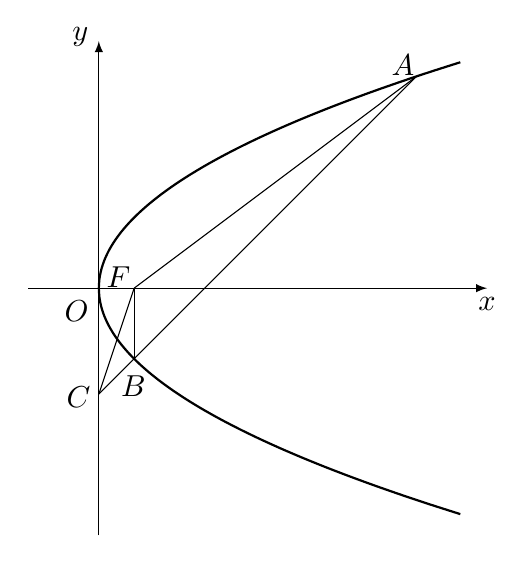
\begin{tikzpicture}[x=1pt, y=1pt,
    every node/.style={inner sep=0pt, font=\fontsize{10.5pt}{12.6pt}\selectfont}]
  \draw[line width=0.398pt] (0.0001,89.2920)   -- (162.2411,89.2920);
  \fill[line width=1.0pt] (165.8277,89.2920)   .. controls (164.7647,89.4910) and (163.0377,90.0890) .. (161.8427,90.7860)   -- (161.8427,87.7980)   .. controls (163.0377,88.4950) and (164.7647,89.0930) .. (165.8277,89.2920);
  \draw[line width=0.398pt] (25.5120,0.0002)   -- (25.5120,174.9972);
  \fill[line width=1.0pt] (25.5120,178.5838)   .. controls (25.3130,177.5208) and (24.7150,175.7938) .. (24.0180,174.5988)   -- (27.0060,174.5988)   .. controls (26.3090,175.7938) and (25.7110,177.5208) .. (25.5120,178.5838);
  \draw[line width=0.797pt] (25.5120,89.2920)   .. controls (25.5120,89.2920) and (25.6130,91.7500) .. (25.7390,92.6940)   .. controls (25.8650,93.6370) and (26.1670,95.1510) .. (26.4190,96.0950)   .. controls (26.6710,97.0390) and (27.1750,98.5530) .. (27.5530,99.4970)   .. controls (27.9300,100.4410) and (28.6370,101.9540) .. (29.1400,102.8980)   .. controls (29.6440,103.8420) and (30.5520,105.3560) .. (31.1810,106.3000)   .. controls (31.8100,107.2440) and (32.9200,108.7570) .. (33.6750,109.7010)   .. controls (34.4310,110.6450) and (35.7420,112.1590) .. (36.6230,113.1030)   .. controls (37.5040,114.0470) and (39.0180,115.5600) .. (40.0250,116.5040)   .. controls (41.0320,117.4480) and (42.7470,118.9620) .. (43.8800,119.9060)   .. controls (45.0120,120.8500) and (46.9300,122.3630) .. (48.1880,123.3070)   .. controls (49.4470,124.2510) and (51.5660,125.7650) .. (52.9500,126.7090)   .. controls (54.3350,127.6530) and (56.6560,129.1670) .. (58.1660,130.1110)   .. controls (59.6770,131.0540) and (62.1990,132.5680) .. (63.8350,133.5120)   .. controls (65.4710,134.4560) and (68.1960,135.9700) .. (69.9580,136.9140)   .. controls (71.7200,137.8570) and (74.6470,139.3710) .. (76.5340,140.3150)   .. controls (78.4220,141.2590) and (81.5500,142.7730) .. (83.5640,143.7170)   .. controls (85.5780,144.6610) and (88.9080,146.1740) .. (91.0470,147.1180)   .. controls (93.1870,148.0620) and (96.7190,149.5760) .. (98.9840,150.5200)   .. controls (101.2490,151.4640) and (104.9830,152.9770) .. (107.3740,153.9210)   .. controls (109.7660,154.8650) and (113.7010,156.3790) .. (116.2180,157.3230)   .. controls (118.7350,158.2670) and (122.8730,159.7800) .. (125.5160,160.7240)   .. controls (128.1590,161.6680) and (132.4980,163.1820) .. (135.2670,164.1260)   .. controls (138.0350,165.0700) and (142.5760,166.5840) .. (145.4710,167.5270)   .. controls (148.3660,168.4710) and (156.1290,170.9290) .. (156.1290,170.9290);
  \draw[line width=0.797pt] (25.5120,89.2920)   .. controls (25.5120,89.2920) and (25.6130,86.8340) .. (25.7390,85.8900)   .. controls (25.8650,84.9470) and (26.1670,83.4330) .. (26.4190,82.4890)   .. controls (26.6710,81.5450) and (27.1750,80.0310) .. (27.5530,79.0870)   .. controls (27.9300,78.1430) and (28.6370,76.6300) .. (29.1400,75.6860)   .. controls (29.6440,74.7420) and (30.5520,73.2280) .. (31.1810,72.2840)   .. controls (31.8100,71.3400) and (32.9200,69.8270) .. (33.6750,68.8830)   .. controls (34.4310,67.9390) and (35.7420,66.4250) .. (36.6230,65.4810)   .. controls (37.5040,64.5370) and (39.0180,63.0240) .. (40.0250,62.0800)   .. controls (41.0320,61.1360) and (42.7470,59.6220) .. (43.8800,58.6780)   .. controls (45.0120,57.7340) and (46.9300,56.2210) .. (48.1880,55.2770)   .. controls (49.4470,54.3330) and (51.5660,52.8190) .. (52.9500,51.8750)   .. controls (54.3350,50.9310) and (56.6560,49.4170) .. (58.1660,48.4730)   .. controls (59.6770,47.5300) and (62.1990,46.0160) .. (63.8350,45.0720)   .. controls (65.4710,44.1280) and (68.1960,42.6140) .. (69.9580,41.6700)   .. controls (71.7200,40.7270) and (74.6470,39.2130) .. (76.5340,38.2690)   .. controls (78.4220,37.3250) and (81.5500,35.8110) .. (83.5640,34.8670)   .. controls (85.5780,33.9230) and (88.9080,32.4100) .. (91.0470,31.4660)   .. controls (93.1870,30.5220) and (96.7190,29.0080) .. (98.9840,28.0640)   .. controls (101.2490,27.1200) and (104.9830,25.6070) .. (107.3740,24.6630)   .. controls (109.7660,23.7190) and (113.7010,22.2050) .. (116.2180,21.2610)   .. controls (118.7350,20.3170) and (122.8730,18.8040) .. (125.5160,17.8600)   .. controls (128.1590,16.9160) and (132.4980,15.4020) .. (135.2670,14.4580)   .. controls (138.0350,13.5140) and (142.5760,12.0000) .. (145.4710,11.0570)   .. controls (148.3660,10.1130) and (156.1290,7.6550) .. (156.1290,7.6550);
  \draw[line width=0.398pt] (25.5120,51.0241)   .. controls (25.5120,51.0241) and (28.9680,54.4801) .. (30.2950,55.8071)   .. controls (31.6230,57.1351) and (33.7520,59.2641) .. (35.0790,60.5911)   .. controls (36.4060,61.9181) and (38.5350,64.0471) .. (39.8620,65.3741)   .. controls (41.1900,66.7021) and (43.3190,68.8311) .. (44.6460,70.1581)   .. controls (45.9730,71.4851) and (48.1020,73.6141) .. (49.4290,74.9411)   .. controls (50.7570,76.2691) and (52.8860,78.3981) .. (54.2130,79.7251)   .. controls (55.5400,81.0521) and (57.6690,83.1811) .. (58.9960,84.5081)   .. controls (60.3240,85.8361) and (62.4530,87.9651) .. (63.7800,89.2921)   .. controls (65.1070,90.6191) and (67.2360,92.7481) .. (68.5630,94.0751)   .. controls (69.8910,95.4031) and (72.0190,97.5311) .. (73.3470,98.8591)   .. controls (74.6740,100.1861) and (76.8030,102.3151) .. (78.1300,103.6421)   .. controls (79.4580,104.9701) and (81.5860,107.0981) .. (82.9140,108.4261)   .. controls (84.2410,109.7531) and (86.3700,111.8821) .. (87.6970,113.2091)   .. controls (89.0250,114.5371) and (91.1530,116.6651) .. (92.4810,117.9931)   .. controls (93.8080,119.3201) and (95.9370,121.4491) .. (97.2640,122.7761)   .. controls (98.5920,124.1041) and (100.7200,126.2321) .. (102.0480,127.5601)   .. controls (103.3750,128.8871) and (105.5040,131.0161) .. (106.8310,132.3431)   .. controls (108.1590,133.6711) and (110.2870,135.7991) .. (111.6150,137.1271)   .. controls (112.9420,138.4541) and (115.0710,140.5831) .. (116.3980,141.9101)   .. controls (117.7260,143.2381) and (119.8540,145.3661) .. (121.1820,146.6941)   .. controls (122.5090,148.0211) and (124.6380,150.1501) .. (125.9650,151.4771)   .. controls (127.2930,152.8051) and (129.4210,154.9331) .. (130.7490,156.2611)   .. controls (132.0760,157.5881) and (134.2050,159.7171) .. (135.5320,161.0441)   .. controls (136.8600,162.3721) and (140.3160,165.8281) .. (140.3160,165.8281);
  \draw[line width=0.398pt] (38.2680,89.2920)   -- (140.3160,165.8280);
  \draw[line width=0.398pt] (38.2680,89.2920)   -- (38.2680,63.7800);
  \draw[line width=0.398pt] (25.5120,51.0240)   -- (38.2680,89.2920);

  \node[anchor=center] at (18.838,180.006) {$y$};  % 源中心 (528.05,779.84)
  \node[anchor=center] at (135.388,169.806) {$A$};  % 源中心 (644.60,769.64)
  \node[anchor=center] at (32.588,93.256) {$F$};  % 源中心 (541.80,693.09)
  \node[anchor=center] at (165.788,83.706) {$x$};  % 源中心 (675.00,683.54)
  \node[anchor=center] at (17.488,81.006) {$O$};  % 源中心 (526.70,680.84)
  \node[anchor=center] at (18.138,50.056) {$C$};  % 源中心 (527.35,649.89)
  \node[anchor=center] at (37.988,53.856) {$B$};  % 源中心 (547.20,653.69)

\end{tikzpicture}
%
% 【自验结果】
%   探针：latexmk -pdfxe（待跑）。
\end{center}
\nopagebreak[4]
(A) \(\dfrac{|BF|-1}{|AF|-1}\)　(B) \(\dfrac{|BF|^2-1}{|AF|^2-1}\)　(C) \(\dfrac{|BF|+1}{|AF|+1}\)　(D) \(\dfrac{|BF|^2+1}{|AF|^2+1}\)

\end{question}
\begin{question}
\gkti{6}设 \(A\)，\(B\) 是有限集，定义：\(d(A,B)=\operatorname{card}(A\cup B)-\operatorname{card}(A\cap B)\)，其中 \(\operatorname{card}(A)\) 表示有限集 \(A\) 中元素的个数。

命题①：对任意有限集 \(A\)，\(B\)，“\(A\neq B\)”是“\(d(A,B)>0\)”的充分必要条件；

命题②：对任意有限集 \(A\)，\(B\)，\(C\)，\(d(A,C)\leqslant d(A,B)+d(B,C)\)。（　）

(A) 命题①和命题②都成立　(B) 命题①和命题②都不成立　(C) 命题①成立，命题②不成立　(D) 命题①不成立，命题②成立

\end{question}
\begin{question}
\gkti{7}存在函数 \(f(x)\) 满足：对于任意 \(x\in\mathbf{R}\) 都有（　）

(A) \(f(\sin 2x)=\sin x\)　(B) \(f(\sin 2x)=x^2+x\)　(C) \(f(x^2+1)=|x+1|\)　(D) \(f(x^2+2x)=|x+1|\)

\Needspace{0.4\textheight}
\end{question}
\begin{question}
\gkti{8}如图，已知 \(\triangle ABC\)，\(D\) 是 \(AB\) 的中点，沿直线 \(CD\) 将 \(\triangle ACD\) 翻折成 \(\triangle A'CD\)，所成二面角 \(A'-CD-B\) 的平面角为 \(\alpha\)，则（　）
\nopagebreak[4]
\begin{center}% f2015zjl_q08_fold.tex — 2015 年高考数学·浙江卷·理科 第 8 题（三角形翻折）
%
% 【来源】`.work/phase3-b19/source/2015浙江理.pdf`（SHA-256
%   801150f0a6d440ac967813d264face6d48b6ee9c69cc20f1c9d6b2b38dec2e9f），
%   第 1 页（合订本页 989）；内容对象 5。逐路径实测见
%   `.work/phase3-b19/figure-inventory.md`。
%
% 【坐标口径】源 PDF 用户空间（原点左下、y 向上）。本图本地坐标
%   (x, y) = (x_page − 532.163, y_page − 239.328)，1 单位 = 1 TeX pt。
%   路径坐标逐点照录内容流（含三次贝塞尔控制点）。
%
% 元素计数：5 条路径（△BDC、A′D、A′C 实线；AD、AC 虚线）＋5 个标签
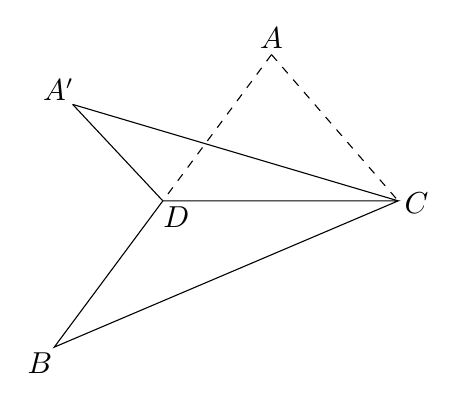
\begin{tikzpicture}[x=1pt, y=1pt,
    every node/.style={inner sep=0pt, font=\fontsize{10.5pt}{12.6pt}\selectfont}]
  \draw[line width=0.398pt] (39.2600,52.8670)   -- (0.0000,0.0000)   -- (124.3000,52.8670)   -- (39.2600,52.8670);
  \draw[line width=0.398pt] (6.6611,87.7336)   -- (39.2601,52.8666);
  \draw[line width=0.398pt] (6.6611,87.7336)   -- (124.3001,52.8666);
  \draw[line width=0.398pt, dash pattern=on 2.989pt off 2.989pt, dash phase=0.0pt] (78.5204,105.7337)   -- (39.2604,52.8667);
  \draw[line width=0.398pt, dash pattern=on 2.989pt off 2.989pt, dash phase=0.0pt] (78.5204,105.7337)   -- (124.3004,52.8667);

  \node[anchor=center] at (78.487,111.712) {$A$};  % 源中心 (610.65,351.04)
  \node[anchor=center] at (1.487,93.012) {$A'$};  % 源中心 (533.65,332.34)
  \node[anchor=center] at (130.887,51.912) {$C$};  % 源中心 (663.05,291.24)
  \node[anchor=center] at (44.087,46.962) {$D$};  % 源中心 (576.25,286.29)
  \node[anchor=center] at (-5.163,-5.888) {$B$};  % 源中心 (527.00,233.44)

\end{tikzpicture}
%
% 【自验结果】
%   探针：latexmk -pdfxe（待跑）。
\end{center}
\nopagebreak[4]
(A) \(\angle A'DB\leqslant\alpha\)　(B) \(\angle A'DB\geqslant\alpha\)　(C) \(\angle A'CB\leqslant\alpha\)　(D) \(\angle A'CB\geqslant\alpha\)

\end{question}
\gkpart{二、填空题}

\begin{question}
\gkti{9}双曲线 \(\dfrac{x^2}{2}-y^2=1\) 的焦距是\gkblank{}，渐近线方程是\gkblank{}。

\end{question}
\begin{question}
\gkti{10}已知函数
\nopagebreak[4]
\[
f(x)=\begin{cases}
x+\dfrac{2}{x}-3, & x\geqslant1,\\
\lg\left(x^2+1\right), & x<1,
\end{cases}
\]
则 \(f(f(-3))=\)\gkblank{}，\(f(x)\) 的最小值是\gkblank{}。

\end{question}
\begin{question}
\gkti{11}函数 \(f(x)=\sin^2x+\sin x\cos x+1\) 的最小正周期是\gkblank{}，单调递减区间是\gkblank{}。

\end{question}
\begin{question}
\gkti{12}若 \(a=\log_4 3\)，则 \(2^a+2^{-a}=\)\gkblank{}。

\Needspace{0.4\textheight}
\end{question}
\begin{question}
\gkti{13}如图，在三棱锥 \(A-BCD\) 中，\(AB=AC=BD=CD=3\)，\(AD=BC=2\)，点 \(M\)，\(N\) 分别为 \(AD\)，\(BC\) 的中点，则异面直线 \(AN\)，\(CM\) 所成的角的余弦值是\gkblank{}。
\nopagebreak[4]
\begin{center}% f2015zjl_q13_tetra.tex — 2015 年高考数学·浙江卷·理科 第 13 题（三棱锥与两中点）
%
% 【来源】`.work/phase3-b19/source/2015浙江理.pdf`（SHA-256
%   801150f0a6d440ac967813d264face6d48b6ee9c69cc20f1c9d6b2b38dec2e9f），
%   第 1 页（合订本页 989）；内容对象 5。逐路径实测见
%   `.work/phase3-b19/figure-inventory.md`。
%
% 【坐标口径】源 PDF 用户空间（原点左下、y 向上）。本图本地坐标
%   (x, y) = (x_page − 918.392, y_page − 615.313)，1 单位 = 1 TeX pt。
%   路径坐标逐点照录内容流（含三次贝塞尔控制点）。
%
% 元素计数：7 条路径（棱 AB/AC/AD/BC/CD 实线、BD 虚线、中线 AN/CM）＋6 个标签
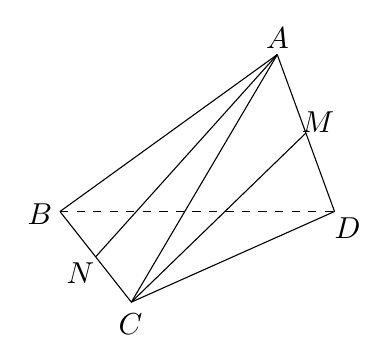
\begin{tikzpicture}[x=1pt, y=1pt,
    every node/.style={inner sep=0pt, font=\fontsize{10.5pt}{12.6pt}\selectfont}]
  \draw[line width=0.398pt] (99.2138,32.7410)   -- (78.5208,89.4350);
  \draw[line width=0.398pt] (0.0000,32.7410)   -- (25.7960,0.0000)   -- (99.2140,32.7410);
  \draw[line width=0.398pt] (78.5206,89.4346)   -- (-0.0004,32.7406);
  \draw[line width=0.398pt] (78.5206,89.4346)   -- (12.8976,16.3706);
  \draw[line width=0.398pt] (25.7957,0.0005)   -- (88.8677,61.0875);
  \draw[line width=0.398pt] (78.5206,89.4346)   -- (25.7956,0.0006);
  \draw[line width=0.398pt, dash pattern=on 2.989pt off 2.989pt, dash phase=0.0pt] (0.0000,32.7410)   -- (99.2140,32.7410);

  \node[anchor=center] at (78.558,95.427) {$A$};  % 源中心 (996.95,710.74)
  \node[anchor=center] at (93.208,65.027) {$M$};  % 源中心 (1011.60,680.34)
  \node[anchor=center] at (-7.242,31.777) {$B$};  % 源中心 (911.15,647.09)
  \node[anchor=center] at (103.958,26.827) {$D$};  % 源中心 (1022.35,642.14)
  \node[anchor=center] at (7.408,10.477) {$N$};  % 源中心 (925.80,625.79)
  \node[anchor=center] at (25.458,-7.973) {$C$};  % 源中心 (943.85,607.34)

\end{tikzpicture}
%
% 【自验结果】
%   探针：latexmk -pdfxe（待跑）。
\end{center}
\nopagebreak[4]
\end{question}
\begin{question}
\gkti{14}若实数 \(x\)，\(y\) 满足 \(x^2+y^2\leqslant1\)，则 \(|2x+y-2|+|6-x-3y|\) 的最小值是\gkblank{}。

\end{question}
\begin{question}
\gkti{15}已知 \(\boldsymbol{e}_1\)，\(\boldsymbol{e}_2\) 是空间单位向量，\(\boldsymbol{e}_1\cdot\boldsymbol{e}_2=\dfrac12\)，若空间向量 \(\boldsymbol{b}\) 满足 \(\boldsymbol{b}\cdot\boldsymbol{e}_1=2\)，\(\boldsymbol{b}\cdot\boldsymbol{e}_2=\dfrac52\)，且对于任意 \(x\)，\(y\in\mathbf{R}\)，\(\left|\boldsymbol{b}-(x\boldsymbol{e}_1+y\boldsymbol{e}_2)\right|\geqslant\left|\boldsymbol{b}-(x_0\boldsymbol{e}_1+y_0\boldsymbol{e}_2)\right|=1\)（\(x_0\)，\(y_0\in\mathbf{R}\)），则 \(x_0=\)\gkblank{}，\(y_0=\)\gkblank{}，\(|\boldsymbol{b}|=\)\gkblank{}。

\end{question}
\gkpart{三、解答题}

\begin{question}
\gkti{16}在 \(\triangle ABC\) 中，内角 \(A\)，\(B\)，\(C\) 所对的边分别是 \(a\)，\(b\)，\(c\)。已知 \(A=\dfrac{\pi}{4}\)，\(b^2-a^2=\dfrac12c^2\)。

（1） 求 \(\tan C\) 的值；

（2） 若 \(\triangle ABC\) 的面积为 \(3\)，求 \(b\) 的值。

\Needspace{0.4\textheight}
\end{question}
\begin{question}
\gkti{17}如图，在三棱柱 \(ABC-A_1B_1C_1\) 中，\(\angle BAC=90^\circ\)，\(AB=AC=2\)，\(A_1A=4\)，\(A_1\) 在底面 \(ABC\) 的射影为 \(BC\) 的中点，\(D\) 是 \(B_1C_1\) 的中点。

（1） 证明：\(A_1D\perp\) 平面 \(A_1BC\)；

（2） 求二面角 \(A_1-BD-B_1\) 的平面角的余弦值。
\nopagebreak[4]
\begin{center}% f2015zjl_q17_prism.tex — 2015 年高考数学·浙江卷·理科 第 17 题（三棱柱）
%
% 【来源】`.work/phase3-b19/source/2015浙江理.pdf`（SHA-256
%   801150f0a6d440ac967813d264face6d48b6ee9c69cc20f1c9d6b2b38dec2e9f），
%   第 2 页（合订本页 990）；内容对象 23。逐路径实测见
%   `.work/phase3-b19/figure-inventory.md`。
%
% 【坐标口径】源 PDF 用户空间（原点左下、y 向上）。本图本地坐标
%   (x, y) = (x_page − 259.718, y_page − 561.951)，1 单位 = 1 TeX pt。
%   路径坐标逐点照录内容流（含三次贝塞尔控制点）。
%
% 元素计数：13 条路径（8 实＋5 虚）＋7 个标签
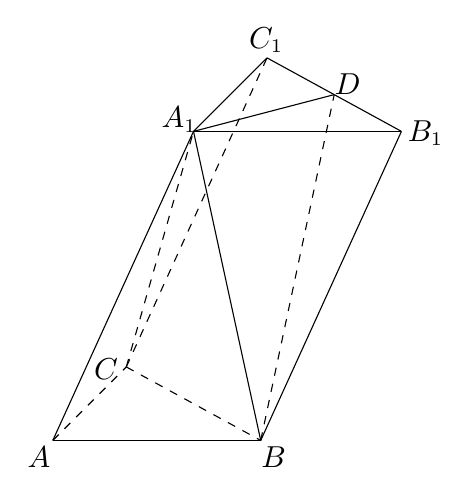
\begin{tikzpicture}[x=1pt, y=1pt,
    every node/.style={inner sep=0pt, font=\fontsize{10.5pt}{12.6pt}\selectfont}]
  \draw[line width=0.3985pt] (0.0000,0.0000)   (0.0000,0.0000)   -- (75.1352,0.0000);
  \draw[line width=0.3985pt] (75.1352,0.0000)   (75.1352,0.0000)   -- (50.8477,111.6752);
  \draw[line width=0.3985pt] (50.8477,111.6752)   (50.8477,111.6752)   -- (125.9829,111.6752);
  \draw[line width=0.3985pt] (125.9829,111.6752)   (125.9829,111.6752)   -- (77.4080,138.2355);
  \draw[line width=0.3985pt] (77.4080,138.2355)   (77.4080,138.2355)   -- (50.8477,111.6752);
  \draw[line width=0.3985pt] (75.1352,0.0000)   (75.1352,0.0000)   -- (125.9829,111.6752);
  \draw[line width=0.3985pt] (0.0000,0.0000)   (0.0000,0.0000)   -- (50.8477,111.6752);
  \draw[line width=0.3985pt] (101.6955,124.9553)   (101.6955,124.9553)   -- (50.8477,111.6752);
  \draw[line width=0.3985pt, dash pattern=on 2.98883pt off 2.98883pt, dash phase=0.0pt] (75.1352,0.0000)   (75.1352,0.0000)   -- (101.6955,124.9553);
  \draw[line width=0.3985pt, dash pattern=on 2.98883pt off 2.98883pt, dash phase=0.0pt] (0.0000,0.0000)   (0.0000,0.0000)   -- (26.5603,26.5603);
  \draw[line width=0.3985pt, dash pattern=on 2.98883pt off 2.98883pt, dash phase=0.0pt] (26.5603,26.5603)   (26.5603,26.5603)   -- (77.4080,138.2355);
  \draw[line width=0.3985pt, dash pattern=on 2.98883pt off 2.98883pt, dash phase=0.0pt] (26.5603,26.5603)   (26.5603,26.5603)   -- (50.8477,111.6752);
  \draw[line width=0.3985pt, dash pattern=on 2.98883pt off 2.98883pt, dash phase=0.0pt] (26.5603,26.5603)   (26.5603,26.5603)   -- (75.1352,0.0000);

  \node[anchor=center] at (77.132,144.589) {$C_1$};  % 源中心 (336.85,706.54)
  \node[anchor=center] at (106.482,128.889) {$D$};  % 源中心 (366.20,690.84)
  \node[anchor=center] at (45.682,115.989) {$A_1$};  % 源中心 (305.40,677.94)
  \node[anchor=center] at (134.682,111.039) {$B_1$};  % 源中心 (394.40,672.99)
  \node[anchor=center] at (19.232,25.589) {$C$};  % 源中心 (278.95,587.54)
  \node[anchor=center] at (-4.968,-5.911) {$A$};  % 源中心 (254.75,556.04)
  \node[anchor=center] at (79.782,-5.911) {$B$};  % 源中心 (339.50,556.04)

\end{tikzpicture}
%
% 【自验结果】
%   探针：latexmk -pdfxe（待跑）。
\end{center}
\nopagebreak[4]
\end{question}
\begin{question}
\gkti{18}\looseness=-1 已知函数 \(f(x)=x^2+ax+b\)（\(a,b\in\mathbf{R}\)），记 \(M(a,b)\) 是 \(|f(x)|\) 在区间 \([-1,1]\) 上的最大值。

（1） 证明：当 \(|a|\geqslant2\) 时，\(M(a,b)\geqslant2\)；

（2） 当 \(a\)，\(b\) 满足 \(M(a,b)\leqslant2\) 时，求 \(|a|+|b|\) 的最大值。

\Needspace{0.4\textheight}
\end{question}
\begin{question}
\gkti{19}已知椭圆 \(\dfrac{x^2}{2}+y^2=1\) 上两个不同的点 \(A\)，\(B\) 关于直线 \(y=mx+\dfrac12\) 对称。

（1） 求实数 \(m\) 的取值范围；

（2） 求 \(\triangle AOB\) 面积的最大值（\(O\) 为坐标原点）。
\nopagebreak[4]
\begin{center}% f2015zjl_q19_ellipse.tex — 2015 年高考数学·浙江卷·理科 第 19 题（椭圆与对称弦）
%
% 【来源】`.work/phase3-b19/source/2015浙江理.pdf`（SHA-256
%   801150f0a6d440ac967813d264face6d48b6ee9c69cc20f1c9d6b2b38dec2e9f），
%   第 2 页（合订本页 990）；内容对象 23。逐路径实测见
%   `.work/phase3-b19/figure-inventory.md`。
%
% 【坐标口径】源 PDF 用户空间（原点左下、y 向上）。本图本地坐标
%   (x, y) = (x_page − 599.627, y_page − 586.119)，1 单位 = 1 TeX pt。
%   路径坐标逐点照录内容流（含三次贝塞尔控制点）。
%
% 元素计数：9 条路径（x/y 轴＋箭头、椭圆、对称轴、OA/OB/AB）＋5 个标签
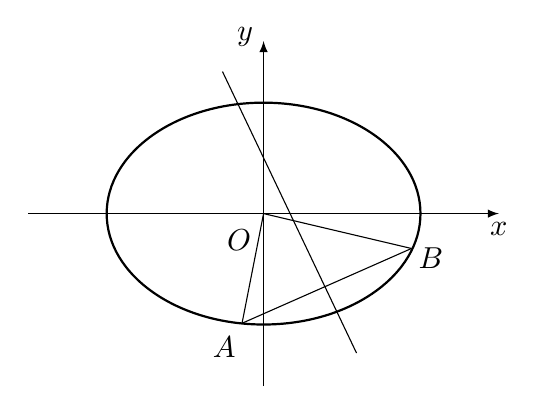
\begin{tikzpicture}[x=1pt, y=1pt,
    every node/.style={inner sep=0pt, font=\fontsize{10.5pt}{12.6pt}\selectfont}]
  \draw[line width=0.3985pt] (-0.0004,62.3630)   -- (166.4939,62.3630);
  \fill[line width=0.3985pt] (170.0804,62.3630)   .. controls (169.0177,62.5622) and (167.2909,63.1600) .. (166.0954,63.8574)   -- (166.0954,60.8686)   .. controls (167.2909,61.5660) and (169.0177,62.1637) .. (170.0804,62.3630);
  \draw[line width=0.3985pt] (85.0400,0.0001)   -- (85.0400,121.1393);
  \fill[line width=0.3985pt] (85.0400,124.7259)   .. controls (84.8408,123.6632) and (84.2430,121.9363) .. (83.5456,120.7408)   -- (86.5344,120.7408)   .. controls (85.8370,121.9363) and (85.2393,123.6632) .. (85.0400,124.7259);
  \draw[line width=0.79701pt] (85.0400,62.3630)   (141.7336,62.3630)   .. controls (141.7336,84.5002) and (116.3514,102.4454) .. (85.0400,102.4454)   .. controls (53.7286,102.4454) and (28.3464,84.5002) .. (28.3464,62.3630)   .. controls (28.3464,40.2258) and (53.7286,22.2806) .. (85.0400,22.2806)   .. controls (116.3514,22.2806) and (141.7336,40.2258) .. (141.7336,62.3630)   -- cycle   (85.0400,62.3630);
  \draw[line width=0.3985pt] (85.0400,62.3630)   -- (138.4822,49.7545);
  \draw[line width=0.3985pt] (85.0400,62.3630)   -- (77.2617,22.7287);
  \draw[line width=0.3985pt] (118.6253,11.9736)   -- (70.1862,113.6905);
  \draw[line width=0.3985pt] (77.2617,22.7287)   -- (138.4822,49.7545);

  \node[anchor=center] at (78.373,126.121) {$y$};  % 源中心 (678.00,712.24)
  \node[anchor=center] at (76.173,52.721) {$O$};  % 源中心 (675.80,638.84)
  \node[anchor=center] at (70.873,13.921) {$A$};  % 源中心 (670.50,600.04)
  \node[anchor=center] at (170.073,56.771) {$x$};  % 源中心 (769.70,642.89)
  \node[anchor=center] at (145.473,46.371) {$B$};  % 源中心 (745.10,632.49)

\end{tikzpicture}
%
% 【自验结果】
%   探针：latexmk -pdfxe（待跑）。
\end{center}
\nopagebreak[4]
\end{question}
\begin{question}
\gkti{20}已知数列 \(\{a_n\}\) 满足 \(a_1=\dfrac12\) 且 \(a_{n+1}=a_n-a_n^2\)（\(n\in\mathbf{N}^*\)）。

（1） 证明：\(1\leqslant\dfrac{a_n}{a_{n+1}}\leqslant2\)（\(n\in\mathbf{N}^*\)）；

（2） 设数列 \(\{a_n^2\}\) 的前 \(n\) 项和为 \(S_n\)，证明：\(\dfrac{1}{2(n+2)}\leqslant\dfrac{S_n}{n}\leqslant\dfrac{1}{2(n+1)}\)（\(n\in\mathbf{N}^*\)）。

\end{question}